\section{Image stitching [35 points]}


In this part you will implement the RANSAC algorithm to stitch two images. The input to the algorithm are two images which are related by an unknown transformation. You will use your blobs detector implemented in the first part to extract keypoints and extract feature descriptors on them.  Your goal is to estimate an affine transformation using feature matching and RANSAC to produce a combined image. 




Recall that the overall steps in the alignment algorithm are:
\begin{enumerate}
\item Detect keypoints in each image (part 1).
\item Extract SIFT features at each detected keypoints.
\item Match features based on pairwise distance.
\item Use RANSAC to estimate the best affine transformation.
\item Stitch the two images using the estimated transformation.
\end{enumerate}


The provided codebase contains an implementation of Step 2 and Step 5. You will implement the remaining steps. The entry code for this homework is in \cmd{evalStitching}.  The code loads two images which contain overlapping areas. Figure~\ref{fig:inputs} shows the "hill" example included in the homework. More test examples are given in the \cmd{data/stitching} folder.




\begin{figure}[h]
\centering
\begin{tabular}{cc}
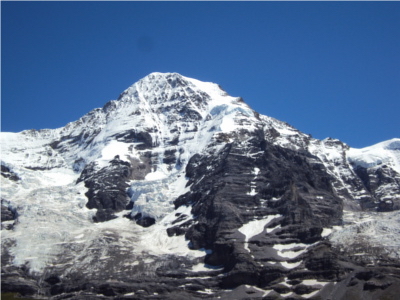
\includegraphics[width=0.45\linewidth]{./fig/hill1.jpg} &
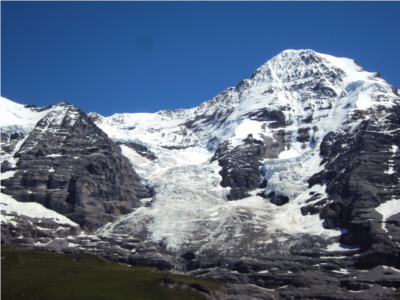
\includegraphics[width=0.45\linewidth]{./fig/hill2.jpg} \\
\end{tabular}
\caption{\label{fig:inputs} Input images to the image stitching algorithm.}
\end{figure}




Below is an outline of the steps you need to implement the algorithm.


\begin{enumerate}


\item \textbf{[0 points] Detect keypoints} The first step is to detect blobs in each image independently. You already implemented this in the first part. Remember to set the initial scale and threshold accordingly to get enough keypoints.
      
\item \textbf{[0 points] Feature extraction.} The next step is to extract feature descriptors on detected keypoints. The code to compute SIFT is included in the code base. The file \cmd{computeSift} takes an image and (x, y, radius) of $N$ blobs as input and return a matrix of size $N \times 128$ with 128 dimensional SIFT descriptor in each row.
%If you are using Matlab, the function uses different external libraries which are included in \cmd{mex} folder depending on the operating system. The first few lines in \cmd{evalStitching.m} sets up the environment variables in Matlab based on your operating system. The code has been tested to work on MATLAB 2019a version and earlier, and should work out of the box on Windows, MAC, and Linux platforms. Talk to the TA in case the mex files are not compatible with your operating system. If you are using Python, just install \cmd{opencv} using your favorite package manager.


\item \textbf{[10 points] Computing matches.} The next step is to compute matches between the two sets of features. Implement the function \cmd{matches = computeMatches(f1,f2)} that returns the best match of each feature \cmd{f1} to \cmd{f2} using the smallest sum-of-squared-differences. The input are two matrices \cmd{f1=dxN} and \cmd{f2=dxM} and the output is a array of size \cmd{Nx1} where each entry \cmd{matches(i)$\in$ [0,1,$\dots$,M]} is the closest feature in \cmd{f2} to the $i^{th}$ feature \cmd{f1(:,i)}, with \cmd{matches(i) = -1} indicating no matching.
%(using MATLAB's 1-starting indexing; for Python a no-match can be indicated by -1).


Considering only nearest neighbors returns many false matches. To refine the matches, compute the ratio of distance from the closest feature to the distance from the second closest feature and reject the matches with the ratio greater than a threshold. \href{http://www.cs.ubc.ca/~lowe/papers/ijcv04.pdf}{David Lowe's paper} suggest a threshold 0.8. Set \cmd{matches(i)=-1} if $i^{th}$ feature \cmd{f1(:,i)} fails on the ratio test.


You can visualize the matches using the \cmd{showMatches(im1, im2, c1, c2, matches)} function provided in the codebase. Figure~\ref{fig:match} shows the output of my implementation for reference.


\begin{figure}[h]
\centering
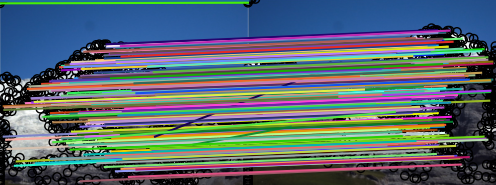
\includegraphics[width=0.75\linewidth]{./fig/matched.jpg}
% \vspace{-0.6in}
\caption{\label{fig:match} Matches between features.}
\end{figure}


\item \textbf{[25 points] Estimating affine transformation using \href{https://en.wikipedia.org/wiki/Random_sample_consensus}{RANSAC}.} The matching in the previous step is noisy and contains many outliers. Using RANSAC, estimate the affine translation that agrees with most matches (inliers). Implement the function \cmd{[inliers, transf] = ransac(matches, c1, c2)}. Here inliners is the indices of the inliner matches, transf is the estimated affine translation of $2\times 3$ matrix \cmd{$[m_1, m_2, t_1; m_3, m_4, t_2]$} between c1 and c2 (here they are blobs1 and blobs2 for image 1 and 2, repectively). You need at least three pairs of points to estimate the this. 

In Python, you might want to use \cmd{cv2.estimateAffine2D} in your implementation.

You can visualize the inlier matches using the \cmd{showMatches} function. Figure~\ref{fig:ransac_result} shows the output of my implementation for reference. The estimated affine transformation for this example is given as follows for your reference:


\begin{center}
$\begin{bmatrix}
0.9683 &  -0.0025 & -124.1000 \\
0.0103 & 0.9866 & 20.6513 \\
\end{bmatrix}$
\end{center}


\begin{figure}[h]
\centering
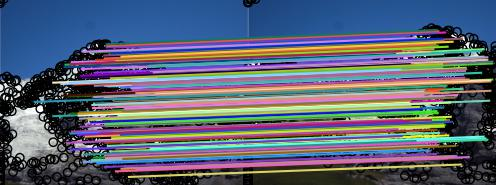
\includegraphics[width=0.75\linewidth]{./fig/ransac_result.jpg}
% \vspace{-0.6in}
\caption{\label{fig:ransac_result} Inliers obtained from RANSAC.}
\end{figure}


\begin{figure}[h]
\centering
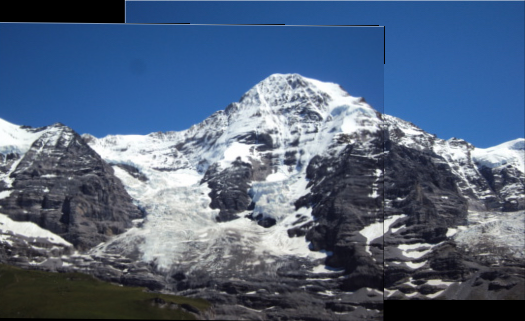
\includegraphics[width=0.8\linewidth]{./fig/stitch_result.jpg}
% \vspace{-0.6in}
\caption{\label{fig:output} Visualization of output.}
\end{figure}
\item \textbf{[0 points] Visualizing the stitched image.} Merge the images using \cmd{mergeImages(im1,im2, transf)} function provided in the codebase. The result is shown as Figure~\ref{fig:output}.
\end{enumerate}

\subsection{What to submit}
To get full credit for this part you have to
\begin{itemize}
\item Include your implementation of \cmd{computeMatches} and \cmd{ransac}.
\item Visualize the intermediate results and the output of each of the provided test image pairs. You can do this by setting the \cmd{exampleIndex} variable in the \cmd{evalStitching} file.
\item Report the estimated affine transformation for given test images.
\end{itemize}







 
